\chapter{State-of-the-Art}
\label{ch:state_of_the_art}

This chapter describes the theoretical foundations, defines the concept of
Strong Eventual Consistency (SEC), and presents two approaches of CRDTs:
state-based, or Convergent Replicated Data Types (CvRDT), and operation-based,
or Commutative Replicated Data Types (CmRDT). Formal specifications for some
examples of data structures are given. The chapter concludes with other
approaches to achieve consistency in the context of data replication, previous
work on CRDTs, and a brief description of a widely used, scalable data store.

\section{Objects, Operations, and Replication}
\label{sec:objects_operations_and_replication}

The following system model was originally introduced in
\cite{shapiro:inria-00555588} and \cite{Shapiro:2011:CRD:2050613.2050642}. 

For our purposes we consider a system consisting of processes which can
communicate in an asynchronous manner over a fully meshed network. The
connection between two processes may drop and recover at any time without
notification. The processes may also crash and recover with their memory intact.

\textit{Objects} are mutable replicated data types. An object has:
\begin{enumerate}[(a)]
  \item an identity;
  \item a content, called its \textit{payload}, which may have any number of
  immutable primitive data types (integers, strings, sets, tuples, etc.) or
  other objects;
  \item an initial state;
  \item an interface which defines the \textit{operations} supported by the
  object.
\end{enumerate}

Two objects having the same identity, but located in different processes are
called \textit{replicas} of each other. Without loss of generality, the
replication of one object across all processes will be considered.

Clients can query and modify the state of an object by calling the operations in
its interface against a replica, called the \textit{source} replica. Queries
execute only locally, i.e. entirely by the corresponding source process.
Operations which modify the state, or update operations, execute in two phases.
In the first phase, called \textit{at-source}, operations are executed
atomically at the source to perform some initial processing, assuming that the
\textit{source precondition} is satisfied (e.g. an element can be removed from a
replicated set only if it is present in the set at the source). If the
precondition is met, then the operation is said to be \textit{enabled} and can
execute as soon as it is invoked. Preconditions may be omitted if the operation
can be always executed. In the second phase, called \textit{downstream}, the
update is transmitted asynchronously from source to all other replicas. With
regards to this, there are two styles of replication recognized by the
literature~\cite{Saito:2005:OR:1057977.1057980}: state-based and
operation-based, explained below.

\section{State-based Replication}
\label{sec:state-based_replication}

In the \textit{state-based} replication style, each update operation is executed
entirely at the source replica, modifying its state. Subsequently, every replica
occasionally sends its local state to some other replica, which \textit{merges}
it into its own state. In this way, every update eventually reaches every
replica directly or indirectly. This process is illustrated in
Figure~\ref{fig:state_based_repl}.

\begin{figure}
  \centering
  \begin{minipage}{0.45\linewidth}
    \centering
    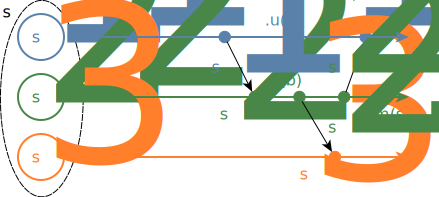
\includegraphics[width=1\textwidth]{state-based-repl}
    \caption{State-based replication}
    \label{fig:state_based_repl}
  \end{minipage}
  \qquad
  \begin{minipage}{0.45\linewidth}
    \centering
    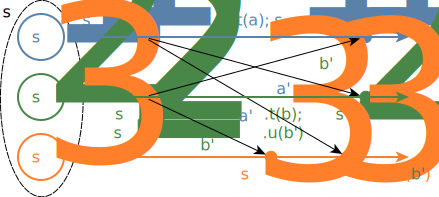
\includegraphics[width=1\textwidth]{op-based-repl}
    \caption{Op-based replication}
    \label{fig:op_based_repl}
  \end{minipage}
\end{figure}

An object is represented as a tuple $(S, s^{0}, f)$, where $S$ is the set of
possible states, $s \in S$ is the current state, or \textit{payload} (initial
state is $s^{0}$), and $f$ can be any of $q$ - \textit{query}, $u$ -
\textit{update}, or $m$ - \textit{merge} operations. The notation $f_{i}^{k}(a)$
refers to the $k^{\text{th}}$ execution of method $f$ with arguments $a$ at
replica $i$. The position of operation $f$ in the time-ordered sequence of all
executions $f$ at replica $i$ is denoted by $K_{i}(f)$. Thus
$K_{i}(f_{j}^{k}(a)) = k$ if $i = j$ and not defined otherwise. Every
$k^{\text{th}}$ update operation $u$ at replica $i$, changes the state from
$s_{i}^{k-1}$ to $s_{i}^{k}$ through the transition $s_{i}^{k} = s_{i}^{k-1}
\bullet f_{i}^{k}(a)$. Queries do not change the state, i.e. if $s' = s \bullet
q$, then $s' \equiv s$, meaning that states $s'$ and $s$ are equivalent (all
queries return the same results for both).

\begin{definition}[\textbf{Casual history -- state-based}]
\label{def:casual_history_state-based}
\begin{itshape}
Causal history for an object is defined as the series $H =
[h_{1},\ldots,h_{n}]$, where $h_{i}$ denotes the history of update operations at
replica $i$: $h_{i} = [h_{i}^{0},\ldots,h_{i}^{k},\ldots]$. Initially,
$h_{i}^{0} = \varnothing$ for all replicas $i = 1,\ldots,n$. If the
$k^{\text{th}}$ execution of an operation at $i$ is: i) a query $q$, then the
causal history does not change, $h_{i}^{k} = h_{i}^{k-1}$; ii) an update $u$,
then it is added to the causal history, $h_{i}^{k} = h_{i}^{k-1} \cup
{u_{i}^{k}(a)}$; iii) a merge $m$ with a remote state $s_{i'}^{k'}$, then the
remote causal history is added to the local one, $h_{i}^{k} = h_{i}^{k-1} \cup
h_{i'}^{k'}$.
\end{itshape}
\end{definition}

An update is said to be \textit{delivered} at some replica if it is included in
that replica's causal history. An update $u$ \textit{happens-before} another
update $u'$ if at the time of execution of $u'$, $u$ is already delivered at
that replica: $u_{i} \rightarrow u'_{i} \iff u_{i} \in h_{i}^{k-1} \land
K_{i}(u'_{i}) \geq k$. Two updates are \textit{concurrent} if no one happens
before the other: $u \parallel u' \iff u \not\rightarrow u' \land u'
\not\rightarrow u$.

In order to have consistency among all replicas, the system has to
deliver every update to every replica. Intuitively, process $i$ sends its state
$s_{i}$ to process $j$. Here, $s_{i}$ is merged into $s_{j}$ by applying method
$m$. We do this infinitely often and choose which replica to send the updates to
according to any algorithm we desire. There are well known protocols in the
literature that do this in a fault-tolerant manner, such as gossip or
anti-entropy~\cite{Demers:1987:EAR:41840.41841,
Petersen:1997:FUP:268998.266711}, which ensure eventual distribution of all
updates in the system.

\section{Operation-based (Op-based) Replication}
\label{sec:operation-based_replication}

In the \textit{operation-based} approach (\textit{op-based} for short), the
system transmits only update operations across replicas, and not whole states,
as illustrated in Figure~\ref{fig:op_based_repl}. In this case, the
\textit{at-source} phase has no side-effects. When it terminates, the system
sends the update operation, its parameters, and possible intermediary results
from the first phase to all replicas, including the source. Here, in downstream,
the operation is executed immediately at source and asynchronously at all other
replicas if the downstream precondition is met. This second phase cannot return
results and has to execute atomically.

Because an op-based object does not have a merge operation, the update
method is split into $(t,u)$ pair, where $t$ is the \textit{prepare-update}
method which has no side-effects and $u$ is the \textit{effect-update} method.
We also require that $u$ follows immediately after $t$, i.e. if $f_{i}^{k-1} =
t$, then $f_{i}^{k} = u$. As explained above, $t$ executes only at the source
replica and does not modify the state, while $u$ executes at all replicas.

\begin{definition}[\textbf{Casual history -- op-based}]
\begin{itshape}
Similar to state-based replication, the initial history is empty at all
replicas: $h_{i}^{0} = \varnothing$. Queries do not change the causal history.
After executing the update $u_{i}^{k}(a)$ at replica $i$ in downstream, it is
added to the local causal history, $h_{i}^{k} = h_{i}^{k-1} \cup
{u_{i}^{k}(a)}$.
\end{itshape}
\end{definition}

As in the state-based case, it is required that all updates eventually reach
the causal history of all replicas. This means we need a reliable broadcast
communication system that delivers every update in an order $<_{d}$, called
\textit{delivery order}, assuming that the downstream precondition holds.
\textit{Causal delivery} $<_{\rightarrow}$ can be thus defined as follows:
$(t,u) \rightarrow (t',u') \iff u \in h_{i}^{k-1}$, where $t'$ executes at
replica $i$, and $K_{i}(t') \geq k$, which means that $u$ is delivered before
$u'$ is delivered and delivery has the same meaning as for state-based objects.
Thus, while related updates are executed in the same sequential order given by
happened-before, concurrent updates (i.e. not ordered by $<_{d}$) may be
delivered in any order. There are common epidemic protocols, such as Bayou's
anti-entropy~\cite{Petersen:1997:FUP:268998.266711}, which provide causal
ordering for updates delivery.

\section{Strong Eventual Consistency (SEC)}
\label{sec:strong_eventual_consistency}

This section gives a formal explanation of what it means for replicas of an
object to eventually converge, or to achieve eventual consistency.

\begin{definition}[\textbf{Eventual Consistency (EC)}]
\begin{itshape}
An object is EC if:
\begin{itemize}
  \item Safety: Replicas that have delivered the same updates, eventually
  reach equivalent states: if $h_{i} = h_{j}, \forall i,j$, then eventually
  $s_{i} \equiv s_{j}$.
  \item Liveness: If an update is delivered at replica $i$, then it is  
  eventually delivered at all replicas $j$: if $u \in h_{i}$, then
  eventually $u \in h_{j}$, $\forall i,j$.
\end{itemize}
\end{itshape}
\end{definition}

Informally, eventual consistency means that all updates are expected to
propagate through the whole system, thus keeping the replicas consistent, given
a sufficiently long period of time in which no updates on the data are applied.
EC implies roll back mechanisms to deal with conflicting updates and consensus
to ensure that all replicas arbitrate conflicts in the same way. A stronger
condition is needed to avoid this:

\begin{definition}[\textbf{Strong Eventual Consistency (SEC)}]
\begin{itshape}
An object is SEC if it is EC and at any time correct replicas that have
delivered the same updates are in equivalent states. 
\end{itshape}
\end{definition}

As mentioned in Section~\ref{sec:motivation_and_problem_definition}, the CAP
theorem states that it is impossible for a distributed system to
simultaneously achieve consistency, availability and network partition
tolerance. Since for most systems nowadays availability cannot be sacrificed,
consistency has to be met through other, weaker constraints. In this context,
SEC provides a solution to this problem, as replicas are always available for
update operations (even if partitioned), while guaranteeing eventual
convergence. However, since the definition implies that all updates are
immediately made persistent, it means that they must have deterministic outcome
which makes this model not universal.

All CRDTs described further in this thesis are proved to achieve SEC, which
gives them some attractive properties: updates can be immediately applied
without taking into account network failures, no distributed consensus and
synchronization for conflict resolution are required, making these data
structures scalable and highly responsive.

\section[State-based CRDT: Convergent Replicated Data Types (CvRDT)]{State-based
CRDT:\\Convergent Replicated Data Types (CvRDT)}
\label{sec:convergent_replicated_data_types}

A \textit{partially ordered set} is the pair consisting in a set together with a
binary relation $\sqsubseteq$ which establishes an order between the elements of
the set. A \textit{least upper bound} (LUB) $\sqcup$ is defined as follows: for
any elements $x$, $y$ from the set, $m = x \sqcup y$ is LUB of $\{x, y\}$ if and
only if $x \sqsubseteq m$ and $y \sqsubseteq m$ and there is no other $m'
\sqsubseteq m$ such that $x \sqsubseteq m'$ and $y \sqsubseteq m'$. From this
definition, it follows that a LUB is: i) commutative: $x \sqcup y = y \sqcup x$,
ii) idempotent: $x \sqcup x = x$, iii) associative: $(x \sqcup y) \sqcup z = x
\sqcup (y \sqcup z)$. A partially ordered set which has a LUB is called a
\textit{join-semilattice}~\cite{semilattice} (or just \textit{semilattice} from
now on). 

An example of semilattice is $(2^{\{x, y, z\}}, \subseteq)$, where $2^{\{x, y,
z\}}$ is the power set of $\{x, y, z\}$ and the LUB is given by set-union.

\begin{definition}[\textbf{Convergent Replicated Data Types (CvRDT)}]
\begin{itshape}
A CvRDT is a state-based object $(S,\sqsubseteq,s^{0},f)$ with the following
properties:
\begin{itemize}
  \item Its payload takes values in the semilattice $(S,\sqsubseteq)$.
  \item Updates monotonically increase the states according to $\sqsubseteq$:
  $s \sqsubseteq s \bullet u$.
  \item The merge operation computes the LUB between the local and remote
  states: $s \bullet m(s') = s \sqcup s'$.
\end{itemize} 
\end{itshape}
\end{definition}

An example of CvRDT can be an object whose payload is an integer value,
$\sqsubseteq$ is common the integer order $\leq$, and where $m()
\stackrel{def}{=} max()$.

In order for a CvRDT to eventually converge, it is required that all replicas
receive all updates. Because the merge operation computes the LUB and is
therefore commutative and idempotent, a reliable communication channel is not
necessary. Messages may be lost, delivered out of order, or multiple time, but
as long as eventually all replicas receive all updates directly or indirectly
via merge operations, convergence is guaranteed.

\begin{theorem}
\begin{itshape}
A state-based object is SEC if it satisfies the CvRDT properties, assuming that
the system transmits updated states infinitely often between all replicas.
\end{itshape}
\end{theorem}

\begin{proof}
We consider any two replicas $i$ and $j$. If $s'_{i} = s_{i} \bullet m(s_{j})$
and $s'_{j} = s_{j} \bullet m(s_{i})$, then, by
Definition~\ref{def:casual_history_state-based}, $s'_{i}$ and $s'_{j}$ will
contain the same causal history, since $h_{i} \cup h_{j} = h_{j} \cup h_{i}$.
Also, because merge computes the LUB and LUB is commutative, we have $s_{i}
\sqcup s_{j} = s_{j} \sqcup s_{i}$ and therefore $s'_{i} = s'_{j}$ in the
semilattice, or $s'_{i} \equiv s'_{j}$. This means that both liveness and safety
properties are maintained and the CvRDT converges towards the LUB of the most
recent updates.
\end{proof}
 
\section[Op-based CRDT: Commutative Replicated Data Types (CmRDT)]{Op-based
CRDT:\\Commutative Replicated Data Types\\(CmRDT)}
\label{sec:commutative_replicated_data_types}

As noted before, in the case of op-based objects a reliable broadcast channel
which delivers all updates at every replica in the delivery order $<_{d}$ is
required. For convergence, another property is needed.

\begin{definition}[\textbf{Commutativity}]
\begin{itshape}
Two updates $(t,u)$ and $(t',u')$ commute if and only if for any reachable
replica in state $s$, where both $u$ and $u'$ are enabled, $u$ (resp. $u'$)
remains enabled in state $s \bullet u'$ (resp. $s \bullet u$) and the resulting
states are equivalent: $s \bullet u \bullet u' \equiv s \bullet u' \bullet u$.
\end{itshape}
\end{definition}

\begin{definition}[\textbf{Commutative Replicated Data Types (CmRDT)}]
\begin{itshape}
A CmRDT is an op-based object for which the following properties hold:
\begin{itemize}
  \item Related updates by happened-before are delivered in the order given by
  $<_{\rightarrow}$.
  \item Concurrent operations commute and may be delivered in any order.
\end{itemize}
\end{itshape}
\end{definition}

\begin{theorem}
\begin{itshape}
An op-based object is SEC if it satisfies the CmRDT properties assuming a
reliable communication channel.
\end{itshape}
\end{theorem}

\begin{proof}
We consider any two replicas $i$ and $j$. Under the assumption of a reliable
broadcast channel, the two replicas will deliver the same operations (if no new
operations are generated) and thus they will have the same causal history,
$h_{i} = h_{j}$. For any two operations $u, v \in h_{i}$: i) if they are not
causally related ($u \parallel v$), then they commute and can be delivered in
any order, i.e. either $K_{i}(u) < K_{i}(v)$ or $K_{i}(u) > K_{i}(v)$; ii) if
they are causally related ($u \rightarrow v$), then they are delivered in the
order $u <_{d} v$ and are applied in the same causal order in both replicas:
$K_{i}(u) < K_{i}(v)$ and $K_{j}(u) < K_{j}(v)$. In all cases an equivalent
abstract state is reached: $h_{i} = h_{j} \Longrightarrow s_{i} \equiv s_{j}$.
\end{proof}

\section{Relation between CvRDTs and CmRDTs}
\label{sec:relation_between_cvrdts_and_cmrdts}

In the previous sections two approaches to eventual convergence were discussed,
in the form of CvRDTs (state-based approach) and CmRDT (op-based approach),
which together are simply called CRDTs. Both of them provide SEC and,
interestingly enough, any data type that can be implemented as a CvRDT can also
be implemented as a CmRDT and vice versa. This equivalence of the two mechanisms
will be formally proved in this section, but first it is necessary to outline
the differences between them and to explain which one is more suitable to be
used depending on the needs.

CvRDTs have the advantage of being simpler to reason about, given that all the
information is captured by their state. Moreover, because this state is
transmitted as part of the merge procedure between two replicas, the
requirements on the communication channel are not strong: messages may be lost
along the way or received in different orders. This also constitutes a
disadvantage because sending whole states is an expensive network operation for
large objects. On the other hand, CmRDTs are more complex to specify since we
need to reason about history and to deliver the updates in a causal-consistent
manner. This puts pressure on the communication channel which has to be reliable
and has to guarantee the same order of message delivery to all replicas. The
advantage comes in the form of a greater expressive power for type specification
(e.g. there is no \textit{merge} method which has to compute a LUB) and smaller
payloads.

\subsection{Op-based Emulation of a State-based Object}
\label{sec:op-based_emulation_of_a_state-based_object}

Any SEC state-based object can be emulated by a SEC op-based object having the
same client interface. Obviously, queries may be ignored because they pose no
problems. Regarding updates, the original $u$ method of the CvRDT is split into
the pair $(t, u')$ of the corresponding CmRDT. For this, it can be considered
that $t(a)$ and $u(a)$ accept the same arguments and return the same values.
Prepare-update method $t(a)$ applies $u(a)$ on a copy of the current replica
state $s$ resulting temporary state $s' = s \bullet u(a)$ and transmits it
further to the client. Here, this state is used as an argument for the
effect-update method $u'(s')$ which delivers it to all replicas by the
underlying protocol of CmRDT and merges it using the original CvRDT merge
method: $s \bullet u'(s') = s \bullet m(s')$. Note that the new update does a
merge and, since merge operations commute for CvRDT, then the update also
commutes. This fact combined with the reliable communication channel assumption
gives us a CmRDT.

\subsection{State-based Emulation of an Op-based Object}
\label{sec:state-based_emulation_of_an_op-based_object}

In order to prove that a SEC op-based object can be emulated as a SEC
state-based object, we consider a CmRDT represented by the tuple $(S, s^{0},
f)$. This can be emulated by a CvRDT object $((S \times U \times U),
\sqsubseteq, (s^{0}, \varnothing, \varnothing), f')$ described next. CvRDT's new
state is now defined as $(s_{m},M,D)$, where $s_{m}$ is the state of the
corresponding original CmRDT. Again, queries can be ignored because they pose no
problems, $(s_{m},M,D) \bullet q'(a) \stackrel{def}{=} (s_{m} \bullet
q(a),M,D)$. For updates, whenever an op-based one is called, it is added to a
set $M$ of received messages to be delivered. In order to avoid duplicate
deliveries, messages which are delivered are stored in a set $D$. Thus, $M$ and
$D$ are grow-only sets. The $\sqsubseteq$ relation is defined by $(s_{m},M,D)
\sqsubseteq (s'_{m},M',D') \stackrel{def}{=} M \subseteq M' \land D \subseteq
D'$. An update $u'(a)$ first calls the original prepare-update method $t(a)$ of
the CmRDT and then the effect-update $u(a)$ locally. It then uses the recursive
function $d$ to process updates:
\[
d(s_{m},M,D) \stackrel{def}{=} 
\begin{cases}
d(s_{m} \bullet u(a),M,D \cup \{u(a)\}), & \text{if }\exists u(a) \in M
\setminus D \\
 (s_{m},M,D), & \text{otherwise}
\end{cases}
\]

Intuitively, $d$ processes any pending updates, i.e. in $M$ but not in $D$.
Therefore, $u'(a)$ will be defined as $(s_{m},M,D) \bullet u'(a)
\stackrel{def}{=} d(s_{m} \bullet t(a),M \cup \{u(a)\},D)$, provided that the
update's downstream precondition is true. Merge operations take the union of
received messages and process available updates: $(s_{m},M,D) \bullet
m(s'_{m},M',D') \stackrel{def}{=} d(s_{m},M \cup M',D)$.

It should be noted that the states of the emulating CvRDT object form a
monotonic semilattice in the domain $S \times U \times U$. Calling or delivering
an operation adds it to the corresponding set and thus advances the state in the
partial order. The \textit{merge} method is defined as the union of sets $M$ and
possibly $D$, and is therefore a LUB operation. After a mutual merge, the $D$
sets in both replicas are identical and their states are equivalent. Also, $M$
contains non-concurrent updates in causal order, while concurrent updates may
appear in any order.

\section{Examples of CRDTs}
\label{sec:examples_of_crdts}

This section gives some concrete examples of CRDTs which are known in the
literature~\cite{shapiro:inria-00555588}. Any of them can be specified
using either the state-based or the op-based approach.

\subsection{Counters}
\label{sec:counters}

The implementation for distributed replicated counters is inspired by vector
clocks. The idea is to consider the counter as a state-based object whose
payload is a vector of integers with the same number of elements as replicas of
that counter, $n$. Thus, the domain where the payload take its values from is
$S = \mathbb{N}^{n}$ and the initial state for all replicas is $s^{0} =
[0,\ldots,0]$. The update operation $inc(i)$ increments the $i^{\text{th}}$
component of the payload, where each process $p_{i}$ is allowed to increment
only its own index $i$: if $s = [s[0],\ldots,s[i],\ldots,s[n-1]]$, then $s
\bullet inc(i) = [s[0],\ldots,s[i] + 1,\ldots,s[n-1]]$. The query $value()$
returns $|s| \stackrel{def}{=} \sum_{i}s[i]$, while the \textit{merge} method
computes the per-index maximum of the two vectors: $s \bullet m(s') =
[max(s[0],s'[0]),\ldots,max(s[n-1],s'[n-1])]$. If we consider the order
operation between these vectors as $s \sqsubseteq s' \iff s[i] \leq s'[i],
\forall i \in \{0,\ldots,n-1\}$, then $(S,\sqsubseteq)$ forms a
monotonic semilattice and merge produces the LUB. Thus this \textbf{increment-only}
counter is a CvRDT.

In order to support decrement operations, two increment-only counters, $I$ and
$D$, can be grouped. Incrementing does an increment on $I$, while decrementing
does an increment in $D$. Now, \textit{value} will return $|I| - |D|$ and
\textit{m} will merge the corresponding counters: $I$ with $I'$ and $D$ with
$D'$. The new partial order is given by $\sqsubseteq$ defined as $(I,D)
\sqsubseteq (I',D') \stackrel{def}{=} I \sqsubseteq I' \land D \sqsubseteq D'$.

\subsection{Registers}
\label{sec:registers}

A register is a memory cell storing a value of any data type and supports
update operation \textit{assign} to change this value and query operation
\textit{value} to retrieve it. Non-concurrent \textit{assign}s are consistent
with sequential semantics: one overwrites the previous one. For concurrent
updates, there are two approaches: either to keep just one (LWW-Register), or to
keep both (MV-Register). 

A \textbf{Last-Writer-Wins Register} (\textbf{LWW-Register}) associates a
unique timestamp to each update to create a total order of assignments
consistent with causal order. This means that for any two assignments, if one
happens before the other, then the first one's timestamp is less than the second
one's. Timestamps can be implemented by concatenating a replica unique ID (such
as MAC address) with a local counter. The usual supported state-based operations
are defined as: the \textit{value} query returns the current value, the
\textit{assign} update assigns a new value to the payload and generates a new
associated timestamp, the \textit{merge} procedure selects the value with the
maximum timestamp. The equivalent op-based \textit{assign} generates the
timestamp at the source in the prepare-update phase and changes the value in the
effect-update phase only if the new timestamp is greater than the old one. This
type of register is found in many distributed systems. One example is
NFS~\cite{Sandberg85designand}, where the LWW-Register represents a file (or a
file block).

The \textbf{Multi-Value Register} (\textbf{MV-Register}) uses a version vector
instead of a timestamp to identify each assignment. The state-based
\textit{assign} method generates a new version vector that is greater than all
existing ones and adds the pair consisting of the new value and the new version
vector to the payload set. The \textit{merge} operation computes the union of
every element in the first set that is not dominated by an element in the second
set. Examples of this type can be found in the Coda file
system~\cite{Howard:1988:SPD:35037.35059} and Amazon's
Dynamo~\cite{DeCandia:2007:DAH:1294261.1294281}.

\subsection{Sets}
\label{sec:sets}

\begin{figure}
  \centering
  \begin{minipage}{1\linewidth}
    \centering
    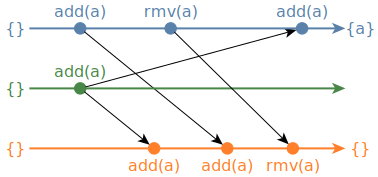
\includegraphics[width=0.45\textwidth]{set-counter-ex}
    \caption{Counter-example for a CRDT set}
    \label{fig:set_counter_ex}
  \end{minipage}
\end{figure}

Sets constitute the building blocks for almost all complex data structures:
containers, maps, and graphs. The supported update operations are \textit{add}
and \textit{remove} which add and, respectively, remove an element to and from
the set. These operations do not commute and, therefore, a CRDT set will be only
an approximation to the sequential specification of a set. Consider the example
in Figure~\ref{fig:set_counter_ex} of a 3-times replicated op-based set.
Initially the set is empty. Replica~1 adds element \textit{a} and then removes
it. Replica~2 adds the same element \textit{a} and sends the update to
Replica~1, thus making $\{a\}$ the final state at Replica~1. Replica~3 receives
both \textit{add} updates from Replica~1 and Replica~2, but only the first one
has effect (adding the same element twice in a set does not change the state).
In the end, Replica~3 receives also the \textit{remove} update from Replica~1,
making $\varnothing$ the final state here. In this example we can see that
although Replica~1 and Replica~3 both applied the operations in causal order,
their states diverge. 

Hence any CRDT implementation of a set can only approximate the sequential set.
The difference is given by having to choose which operation to take precedence
in a concurrent $\textit{add}(e) \parallel \textit{remove}(e)$ situation: either
\textit{remove} wins (the 2P-Set), or \textit{add} wins (the OR-Set).

\begin{algorithm}[t]
\small{
	\floatname{algorithm}{Specification}
	\caption{G-Set (state-based)}
 	\label{alg:g_set_state_based}                       

 	\begin{algorithmic}[1]
 	  \State \Payload $A = \varnothing$
 	  
 	  \State \Update $add(e)$
 	  \State \hspace{\algorithmicindent} $A \coloneqq A \cup \{e\}$
 	  
 	  \State \Query $lookup(e) : \text{boolean}$
 	  \State \hspace{\algorithmicindent} \Return $e \in A$
 	  
 	  \State \Compare $(S, T) : \text{boolean}$
 	  \State \hspace{\algorithmicindent} \Return $S.A \subseteq T.A$
 	  
 	  \State \Merge $(S, T) : \text{payload}$
 	  \State \hspace{\algorithmicindent} \Return $S.A \cup T.A$
	\end{algorithmic}
 }
\end{algorithm}

The first CRDT implementation of a set, \textbf{Grow-Only Set} (\textbf{G-Set}),
allows for \textit{add} and \textit{lookup} operations. Both state-based and
op-based versions have a set as payload. To prove that this is a CmRDT it is
easy to see that $\textit{add}(e)$ is commutative, being based on a set-union
operation between the payload and $\{e\}$. In the state-based approach, as shown in
Specification~\ref{alg:g_set_state_based}, the partial order on states $S$ and
$T$ is given by $S \sqsubseteq T \iff S \subseteq T$. Then, the \textit{merge}
operation defined as $\textit{merge}(S,T) = S \cup T$ computes the LUB in the
monotonic semilattice $(S, \sqsubseteq)$. And so, G-Set is also a CvRDT.

\begin{algorithm}[t]
\small{
	\floatname{algorithm}{Specification}
	\caption{2P-Set (state-based)}
 	\label{alg:2p_set_state_based}                       

 	\begin{algorithmic}[1]
 	  \State \Payload $A = \varnothing, R = \varnothing$
 	  
 	  \State \Update $add(e)$
 	  \State \hspace{\algorithmicindent} $A \coloneqq A \cup \{e\}$
 	  
 	  \State \Update $remove(e)$
 	  \State \hspace{\algorithmicindent} \Pre $lookup(e)$
 	  \State \hspace{\algorithmicindent} $R \coloneqq R \cup \{e\}$
 	  
 	  \State \Query $lookup(e) : \text{boolean}$
 	  \State \hspace{\algorithmicindent} \Return $e \in A \land e \not\in R$
 	  
 	  \State \Compare $(S, T) : \text{boolean}$
 	  \State \hspace{\algorithmicindent} \Return $S.A \subseteq T.A \lor S.R \subseteq T.R$ 
 	  
 	  \State \Merge $(S, T) : \text{payload}$
 	  \State \hspace{\algorithmicindent} \Let $U.A = S.A \cup T.A$
 	  \State \hspace{\algorithmicindent} \Let $U.R = S.R \cup T.R$
 	  \State \hspace{\algorithmicindent} \Return $U$
	\end{algorithmic}
 }
\end{algorithm}

A \textbf{Two-Phase Set} (\textbf{2P-Set}) brings the option to remove an
element. However, once an element has been removed, it cannot be added again to
the set. The principle is to use two G-Sets, one for adding and another for
removing (also known as \textit{tombstone set}). Removing an element is
conditioned by being present in the set at source. The state-based variant is
shown in Specification~\ref{alg:2p_set_state_based}. The payload consists of set
$A$ for adding and set $R$ for removing. Adding or removing the same element
twice or adding an already removed element has no effect. The \textit{merge}
operation computes the LUB of the two sets by applying set-union on each one
individually. Thus, the state-based 2P-Set is a CvRDT. Considering the op-based
approach, concurrent \textit{add} and \textit{remove} operations on same element
and concurrent operations on different elements commute. Also $\textit{add}(e)
\parallel \textit{add}(e)$ and $\textit{remove}(e) \parallel \textit{remove}(e)$
commute by definition. It follows that 2P-Set is also a CmRDT.

\begin{algorithm}[t]
\small{
	\floatname{algorithm}{Specification}
	\caption{U-Set (op-based)}
 	\label{alg:u_set_op_based}                       

 	\begin{algorithmic}[1]
 	  \State \Payload $S = \varnothing$
 	  \State \Query $lookup(e) : \text{boolean}$
 	  \State \hspace{\algorithmicindent} \Return $e \in S$
 	  
 	  \State \Update $add(e)$
 	  \State \hspace{\algorithmicindent} \Prepare $(e)$
 	  \State \hspace{\algorithmicindent}\hspace{\algorithmicindent} \Pre $e$ is unique 
 	  \State \hspace{\algorithmicindent} \Effect $(e)$ 
 	  \State \hspace{\algorithmicindent}\hspace{\algorithmicindent} $S \coloneqq S \cup \{e\}$
 	  
 	  \State \Update $remove(e)$
 	  \State \hspace{\algorithmicindent} \Prepare $(e)$
 	  \State \hspace{\algorithmicindent}\hspace{\algorithmicindent} \Pre $lookup(e))$ 
 	  \State \hspace{\algorithmicindent} \Effect $(e)$ 
 	  \State \hspace{\algorithmicindent}\hspace{\algorithmicindent} \Pre $add(e)$ has been delivered
 	  \State \hspace{\algorithmicindent}\hspace{\algorithmicindent} $S \coloneqq S \setminus \{e\}$
	\end{algorithmic}
 }
\end{algorithm}

If we guarantee that each element in the set is unique\footnote{To achieve
global unique elements across all replicated sets, Lamport clocks can be used or
a function which generates random numbers from a large space.} and that an
$\textit{add}(e)$ is delivered before $\textit{remove}(e)$, the tombstone set
becomes redundant and can be discarded because the causal delivery criteria
is met. This new data structure is called \textbf{U-Set} and it is presented in
Specification~\ref{alg:u_set_op_based}. It is easy to show that the U-Set is a
CmRDT: since each element is unique, \textit{add}s are independent; also there
cannot be concurrent \textit{add} and \textit{remove} on the same element
because each \textit{remove} must casually follow the corresponding
\textit{add}.

An alternative solution, called a \textbf{PN-Set}, is to associate with each
element a CRDT counter (initially set to 0) which is increased when the element
is added to the set and decreased when it is removed. If the counter is
negative, it means that the element is not in the set, and \textit{add}
operation will not have any effect. Thus a PN-Set has the anomaly that after
adding a previously removed element to an empty set, it remains empty. This may
not always be the intended semantics, despite the fact that PN-Set converges (it
combines two CRDTS, a set and a counter).

The previously described set structures, although practical, have
counter-intuitive behaviors. For example, the 2P-Set does not allow adding an
element after it has been removed, while the PN-Set has the problem showed
above. The \textbf{Observed-Removed Set} (\textbf{OR-Set}) introduced in
\cite{preguica:inria-00445758} is closer to the usual set semantics. The idea is
to uniquely tag each added element. When removing an element, only associated
tags observed at the source are removed.

\begin{algorithm}[t]
\small{
	\floatname{algorithm}{Specification}
	\caption{OR-Set (op-based)}
 	\label{alg:or_set_op_based}                       

 	\begin{algorithmic}[1]
 	  \State \Payload $S = \varnothing$
 	  \State \Query $lookup(e) : \text{boolean}$
 	  \State \hspace{\algorithmicindent} \Return $\exists u : (e, u) \in S$
 	  
 	  \State \Update $add(e)$
 	  \State \hspace{\algorithmicindent} \Prepare $(e) : \text{tag}$
 	  \State \hspace{\algorithmicindent}\hspace{\algorithmicindent} \Let $\alpha = unique()$
 	  \State \hspace{\algorithmicindent}\hspace{\algorithmicindent} \Return $\alpha$
 	  \State \hspace{\algorithmicindent} \Effect $(e, \alpha)$ 
 	  \State \hspace{\algorithmicindent}\hspace{\algorithmicindent} $S \coloneqq S \cup \{(e, \alpha)\}$
 	  
 	  \State \Update $remove(e)$
 	  \State \hspace{\algorithmicindent} \Prepare $(e) : \text{set}$
 	  \State \hspace{\algorithmicindent}\hspace{\algorithmicindent} \Pre $lookup(e)$
 	  \State \hspace{\algorithmicindent}\hspace{\algorithmicindent} \Let $R = \{(e, u) \mid \exists u : (e, u) \in S\}$
 	  \State \hspace{\algorithmicindent}\hspace{\algorithmicindent} \Return $R$
 	  \State \hspace{\algorithmicindent} \Effect $(R)$ 
 	  \State \hspace{\algorithmicindent}\hspace{\algorithmicindent} \Pre $\forall (e, u) \in R : add(e, u)$ has been delivered
 	  \State \hspace{\algorithmicindent}\hspace{\algorithmicindent} $S \coloneqq S \setminus R$
	\end{algorithmic}
 }
\end{algorithm}

Specification~\ref{alg:or_set_op_based} describes the usual supported operations
for the op-based variant. The payload is a set of pairs
$(\textit{e},\textit{tag})$. Method $\textit{add}(e)$ generates a new unique tag
at source in the prepare-update phase and then sends it to all replicas which
insert it into their payload in the effect-update phase. In this way, two
additions of the same element are distinguished by their tags, but
\textit{lookup} masks the duplicates. Method $\textit{remove}(e)$ gathers all
tags associated with $e$ at source and sends them to all replicas which remove
the corresponding pairs from their local payloads. Because a
$\textit{remove}(e)$ will only remove locally observed elements, a concurrent
$\textit{add}(e) \parallel \textit{remove}(e)$ will give precedence to
$\textit{add}(e)$, in contrast to the 2P-Set.

This behavior is illustrated in Figure~\ref{fig:or_set_op_based}. Here the two
$\textit{add}(a)$ operations generate unique tags $\alpha$ and $\beta$,
respectively. When Replica~1 applies $\textit{rmv}(a)$, it translates to
removing $(a, \alpha)$ downstream. The $\textit{add}(a)$ at Replica~2 is
concurrent to the $\textit{rmv}(a)$ at Replica~1 and, therefore, $(a, \beta)$
remains in the final state. 

\begin{figure}[b]
  \centering
  \begin{minipage}{1\linewidth}
    \centering
    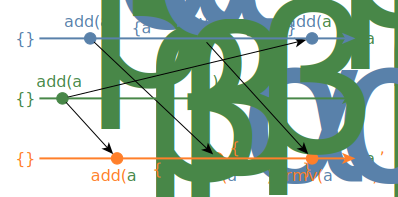
\includegraphics[width=0.45\textwidth]{or-set-op-based}
    \caption{OR-Set (op-based)}
    \label{fig:or_set_op_based}
  \end{minipage}
\end{figure}

OR-Set is a CmCRDT because: i) concurrent \textit{add}s commute since each one is
unique; ii) concurrent \textit{remove}s commute since any common pairs have the
same effect, and any disjoint pairs have independent effects; iii) concurrent
$\textit{add}(e_{1})$ and $\textit{remove}(e_{2})$ commute: if $e_{1} \neq
e_{2}$ they are independent, else \textit{remove} has no effect.

\begin{algorithm}[t]
\small{
	\floatname{algorithm}{Specification}
	\caption{OR-Set (state-based)}
 	\label{alg:or_set_state_based}                       

 	\begin{algorithmic}[1]
 	  \State \Payload $A = \varnothing, R = \varnothing$
 	  \State \Query $lookup(e) : \text{boolean}$
 	  \State \hspace{\algorithmicindent} \Return $\exists \alpha : (e, \alpha) \in A \land \nexists \beta : (a, \alpha, \beta) \in R$
 	  
 	  \State \Update $add(e)$
 	  \State \hspace{\algorithmicindent} \Let $\alpha = unique()$
 	  \State \hspace{\algorithmicindent} $A \coloneqq A \cup \{(e, \alpha)\}$
 	  
 	  \State \Update $remove(e)$
 	  \State \hspace{\algorithmicindent} \Pre $lookup(e)$
 	  \State \hspace{\algorithmicindent} \Let $\beta = unique()$
 	  \State \hspace{\algorithmicindent} \Let $R' = \{(e, \alpha, \beta) | \exists (e, \alpha) \in A\}$
 	  \State \hspace{\algorithmicindent} $R \coloneqq R \cup R'$
 	  
 	  \State \Compare $(S, T) : \text{boolean}$
 	  \State \hspace{\algorithmicindent} \Return $S.A \subseteq T.A \land S.R \subseteq T.R$ 
 	  
 	  \State \Merge $(S, T) : \text{payload}$
 	  \State \hspace{\algorithmicindent} \Let $U.A = S.A \cup T.A$
 	  \State \hspace{\algorithmicindent} \Let $U.R = S.R \cup T.R$
 	  \State \hspace{\algorithmicindent} \Return $U$
	\end{algorithmic}
 }
\end{algorithm}

The state-based approach is presented in
Specification~\ref{alg:or_set_state_based}. Here the payload contains two
sets, $A$ for added elements and $R$ for removed elements. When adding an
element $e$, like in the op-based approach, a new unique tag $\alpha$ is
generated and the pair $(e, \alpha)$ is inserted into the $A$ set. The
\textit{remove} operation again generates a unique tag $\beta$, associates it
with all matching pairs from $A$, and stores the result in the $R$ set. To test
if an element is in the OR-Set, we just need to verify if it is in $A$ and not
in $R$. The partial order on the payload states is given by the relation $S
\sqsubseteq T \iff S.A \subseteq T.A \land S.R \subseteq T.R$. Because update
operations always compute larger states relative to $\sqsubseteq$ and because
\textit{merge} computes the LUB, state-based OR-Set is also a CRDT.

\subsection{Graphs}
\label{sec:graphs}

A graph is defined as a pair of sets $(V, E)$, where $V$ is the set of vertices
and $E \subseteq V \times V$ is the set of edges between vertices. For $V$ and
$E$ any of the set structures previously described can be used. Since we cannot
add an edge if any of the two connecting vertices is missing and we cannot
remove a vertex if it supports an edge, update operations on vertices and edges
are not independent. Therefore an analysis is needed when $\textit{addEdge}(u,
v) \parallel \textit{removeVertex}(u)$. There are three possibilities: i) give
precedence to $\textit{removeVertex}(u)$: all edges to or from $u$ are also
removed, ii) give precedence to $\textit{addEdge}(u, v)$: if either $u$ or $v$
has been removed, it is restored, and iii) $\textit{removeVertex}(u)$ is delayed
until all concurrent $\textit{addEdge}(u, v)$ operations have been executed.

Since option ii) has complex semantics and option iii) requires synchronization,
option i) is presented in Specification~\ref{alg:graph_op_based}. The idea is to
use the same approach as for the OR-Set. The payload contains two sets, one for
vertices and one for edges. Adding a vertex $v$ first generates a unique
identifier $\alpha$ at the source and then adds the pair $(v, \alpha)$ to the
set of vertices in the downstream phase. To remove a vertex $v$, the
prepare-update method computes the set of pairs that contain $v$ at source and
the effect-update method removes this set from the set of vertices in all
replicas. Since we have the guarantee that operations are delivered in the
causal order, we know that for each element to be removed the corresponding
\textit{addVertex} has been called. As with OR-Sets, $\textit{addVertex}(v)$
wins when $\textit{addVertex}(v) \parallel \textit{removeVertex}(v)$ because
$\textit{removeVertex}(v)$ operates only on the locally observed vertices at
source. The same approach is used for adding and removing edges. In order to
avoid the anomalies mentioned in the beginning of the section, preconditions
are used in the prepare phases.

\begin{algorithm}[t!]
\small{
	\floatname{algorithm}{Specification}
	\caption{Directed graph (op-based)}
 	\label{alg:graph_op_based}                       

 	\begin{algorithmic}[1]
 	  \State \Payload $V = \varnothing, E = \varnothing$
 	  
 	  \State \Query $lookupVertex(v) : \text{boolean}$
 	  \State \hspace{\algorithmicindent} \Return $\exists \alpha : (v, \alpha) \in V$
 	  
 	  \State \Query $lookupEdge((v', v'')) : \text{boolean}$
 	  \State \hspace{\algorithmicindent} \Return $lookupVertex(v') \land lookupVertex(v'') \land \exists \alpha : ((v', v''), \alpha) \in E$
 	  
 	  \State \Update $addVertex(v)$
 	  \State \hspace{\algorithmicindent} \Prepare $(v) : \text{tag}$
 	  \State \hspace{\algorithmicindent}\hspace{\algorithmicindent} \Let $\alpha = unique()$
 	  \State \hspace{\algorithmicindent}\hspace{\algorithmicindent} \Return $\alpha$
 	  \State \hspace{\algorithmicindent} \Effect $(v, \alpha)$ 
 	  \State \hspace{\algorithmicindent}\hspace{\algorithmicindent} $V \coloneqq V \cup \{(v, \alpha)\}$
 	  
 	  \State \Update $removeVertex(v)$
 	  \State \hspace{\algorithmicindent} \Prepare $(v) : \text{set}$
 	  \State \hspace{\algorithmicindent}\hspace{\algorithmicindent} \Pre $lookupVertex(v)$
 	  \State \hspace{\algorithmicindent}\hspace{\algorithmicindent} \Pre $\nexists v' : lookupEdge((v, v'))$
 	  \State \hspace{\algorithmicindent}\hspace{\algorithmicindent} \Let $R = \{(v, \alpha) | \exists \alpha : (v, \alpha) \in V\}$
 	  \State \hspace{\algorithmicindent}\hspace{\algorithmicindent} \Return $R$
 	  \State \hspace{\algorithmicindent} \Effect $(R)$ 
 	  \State \hspace{\algorithmicindent}\hspace{\algorithmicindent} $V \coloneqq V \setminus R$
 	  
 	  \State \Update $addEdge(v', v'')$
 	  \State \hspace{\algorithmicindent} \Prepare $(v', v'') : \text{tag}$
 	  \State \hspace{\algorithmicindent}\hspace{\algorithmicindent} \Pre $lookupVertex(v')$
 	  \State \hspace{\algorithmicindent}\hspace{\algorithmicindent} \Let $\alpha = unique()$
 	  \State \hspace{\algorithmicindent}\hspace{\algorithmicindent} \Return $\alpha$
 	  \State \hspace{\algorithmicindent} \Effect $(v', v'', \alpha)$ 
 	  \State \hspace{\algorithmicindent}\hspace{\algorithmicindent} $E \coloneqq E \cup \{((v', v''), \alpha)\}$
 	  
 	  \State \Update $removeEdge(v', v'')$
 	  \State \hspace{\algorithmicindent} \Prepare $(v', v'') : \text{set}$
 	  \State \hspace{\algorithmicindent}\hspace{\algorithmicindent} \Pre $lookupEdge((v', v''))$
 	  \State \hspace{\algorithmicindent}\hspace{\algorithmicindent} \Let $R = \{((v', v''), \alpha) | \exists \alpha : ((v', v''), \alpha) \in E\}$
 	  \State \hspace{\algorithmicindent}\hspace{\algorithmicindent} \Return $R$
 	  \State \hspace{\algorithmicindent} \Effect $(R)$ 
 	  \State \hspace{\algorithmicindent}\hspace{\algorithmicindent} $E \coloneqq E \setminus R$
	\end{algorithmic}
 }
\end{algorithm}

To prove that this op-based specification is a CRDT, it should be shown as
usually that concurrent updates commute. $\textit{addVertex}(v') \parallel
\textit{addVertex}(v'')$ commute as both generate unique tags and perform a
set union, which is a commutative operation. $\textit{removeVertex}(v')
\parallel \textit{removeVertex}(v'')$ commute because they perform $V \setminus
R'$ and $V \setminus R''$, respectively, and $V \setminus R' \setminus R'' = V
\setminus R'' \setminus R'$, where $R'$, $R''$ are the sets of observed vertices
to be removed. $\textit{addVertex}(v') \parallel \textit{removeVertex}(v'')$
also commute because $\textit{addVertex}(v')$ generates a fresh unique $\alpha$,
and therefore $(v', \alpha) \not\in R''$ and $V \cup \{(v', \alpha)\} \setminus
R'' = V \setminus R'' \cup \{(v', \alpha)\}$. For edges, the proof follows the
same steps. Finally, since any concurrent updates on vertices and edges modify
disjoint internal sets, from this it results that they commute too.

As seen, graphs are more complex data structures, but they can be easily
implemented by composing simpler CRDTs, like OR-Sets or 2P-Sets. However,
maintaining a particular shape, such as a tree or a directed acyclic graph
(DAG), cannot be done by a CRDT since this requires synchronization to ensure a
global acyclicity invariant. But types which employ some stronger forms of
acyclicity are viable. In a \textbf{monotonic DAG} an edge may be added only if
it is oriented in the same direction as an existing path, thus strengthening the
partial order defined by the DAG. The specification for this type can be found
in \cite{shapiro:inria-00555588}.

\section{Other Approaches to Consistency}
\label{sec:other_approaches_to_consistency}

The fundamental principles on database replication are laid out
in~\cite{lindsay} and a number of techniques are discussed there to achieve
consistency. The traditional \textit{strong consistency} approach imposes a
global total order on updates to serialize
them~\cite{Lamport:1978:TCO:359545.359563}. This conflicts with availability and
partition-tolerance~\cite{Gilbert:2002:BCF:564585.564601} and leads to
performance and scalability bottlenecks. \textit{Sequential consistency} is
another model, weaker than strong consistency, but undecidable in
practice~\cite{Qadeer:2003:VSC:939835.940001}. A survey on other models is
presented in~\cite{Mosberger:1993:MCM:160551.160553}.

Techniques for achieving eventual consistency for large-scale distributed
systems have been an active focus point in recent research. This is mostly due
to the explosion of Internet-based and peer-to-peer services. However, the
origins of the principles behind CRDTs can be found in the apparent unrelated
area of file systems. The state-based approach was introduced for register-like
objects, where the only operation is assignment. It is widely used in
NFS~\cite{Sandberg85designand}, AFS~\cite{Howard:1988:SPD:35037.35059} and
Coda~\cite{Kistler:1992:DOC:146941.146942} file systems and in key-value stores
such as Amazon's Dynamo~\cite{DeCandia:2007:DAH:1294261.1294281} or
Riak~\cite{riak}. The mathematical foundations were laid by Baquero and
Moura~\cite{scadt4} and later extended by Shapiro and Preguiça on their work on
Treedoc~\cite{Preguica:2009:CRD:1584339.1584604} in order to support the
operation-based approach, thus coining the term of CRDT. Examples of
implementations for this second approach are found in Bayou’s anti-entropy
protocol~\cite{Petersen:1997:FUP:268998.266711} and the IceCube cooperative
system~\cite{preguica:inria-00445758}.

Later, a formal definition and rigorous system model for CRDT were published
in \cite{shapiro:inria-00555588} and \cite{Shapiro:2011:CRD:2050613.2050642}.
These are the first works to engage a comprehensive and systematic study on
CRDTs. The thesis extends these definitions to support an efficient
synchronization algorithm which transmits only deltas of updates and introduces
a specification for partitioning a CRDT OR-Set replica into disjunctive subsets.
A garbage collection mechanism to reclaim obsolete elements from the set is also
discussed. On the practical side, to the author's knowledge, this is the first
implementation of a CRDT in the sense of the system model described in this
chapter. Proof-of-concept examples exists~\cite{ericmoritz, dominictarr}, but
they focus only on testing the specifications for CRDTs locally and in-memory,
without a real database store support. ConcoRDanT~\cite{concordant} is an
interesting project aimed to investigate the principles of these types.

\section{Short Introduction on Redis}
\label{sec:short_introduction_on_redis}

NoSQL is a class of database management systems introduced as an alternative to
traditional RDMBSs in order to cope with problems of certain data models, such
as low throughput, unneeded complexity, and horizontal scalability~\cite{nosql}.
Representatives of this class of applications compensate the lack of advanced
features with gains in scalability and performance.

In this sense, Redis~\cite{redis} is a widely used, open-source, in-memory,
key-value store with many features which make it an ideal database system for
evaluating the contributions of this thesis as shown in
Chapter~\ref{ch:implementation_and_evaluation}. Its data model is a dictionary
that maps keys to values. All the following data types are supported:

\begin{itemize}
  \item \textit{Strings}: the most basic data type, binary safe and can contain
  any kind of data. Redis also allows a number of interesting operations to be
  applied to strings: consider them as integers and increment or decrement them
  atomically, append to them, use them as random access vectors to get a
  substring or encode a lot of binary data and accessing bits of it at given
  offsets.
  \item \textit{Lists}: simply lists of strings, sorted by insertion order.
  Accessing elements is very fast near the extremes of the list,
  $\mathcal{O}(1)$ at the head (on the left) or at the tail (on the right), but
  is slow in the middle of a very big list, $\mathcal{O}(N)$.
  \item \textit{Sets}: unordered non repeating collection of strings. They
  support operations to add, remove, and test for existence of members in
  $\mathcal{O}(1)$ time.
  \item \textit{Sorted sets}: similar to sets but where every element is
  associated to a floating number score and the elements are sorted by this
  score. Usual operations take $\mathcal{O}(log(N))$ time.
  \item \textit{Hashes}: maps between string fields and string values, can
  also be seen as collections of (field, value) pairs. They are suitable for
  storing objects: the key can represent the object id, while the fields can
  represent the attributes.
\end{itemize}

The keys in Redis can be only strings, while as values all the above data
types are supported. Other Redis features include persistence, replication,
transactions, pipelining, or Lua scripts. In addition, Redis has support for
associating timeouts with keys. After the timeout has expired, the key is
automatically deleted. Some of these features match perfectly with the design
from Chapter~\ref{ch:design_of_sharded_or-set}. For a complete documentation,
the reader is referred to the Redis website~\cite{redis}.
